\chapter{Autoskalowanie}
\label{cha:autoscaling}

\cw{Cluster} SurfAdvisor skaluje się w dwóch wymiarach:

\begin{itemize}
    \item
    \cw{Pod} - \textbf{Horizontal Pod Autoscaling}\\
    ilość \cw{Pod}'ów \emph{(instancji)} danej aplikacji
    \item
    \cw{Node} - \textbf{Horizontal Node Autoscaling}\\
    ilość \cw{Node}'ów \emph{(wirtualnych maszyn)} składających się na \cw{Cluster}
\end{itemize} 

\section{Horizontal Pod Autoscaling}

Autoskalowanie \cw{Pod}'ów definiuje się poprzez skojarzony obiekt \cw{HorizontalPodAutoscaler}.
Kluczowe znaczenie mają właściwości:

\begin{itemize}
    \item
    minimalna ilość \cw{Pod}'ów
    \item
    maksymalna ilość \cw{Pod}'ów
    \item
    metryka, która wzbudza skalowanie
\end{itemize} 

Aby skalowanie było możliwe, definicja \cw{Pod}'a musi zawierać wymagania co do zużycia zasobów \emph{(CPU, RAM)}.

Działanie autoskalowania zaprezentowane zostanie podczas testu obciążeniowego \emph{dictionary-service}.
W stanie spoczynkowym liczba \cw{Pod}'ów tego \cw{Service}'u wynosi \textbf{1}, maksymalnie może osiągnąć \textbf{10}, 
skalowanie wzbudzane jest przekroczeniem \textbf{50\%} zużycia \textbf{CPU}.

\begin{figure}[!ht]
	\begin{center}
		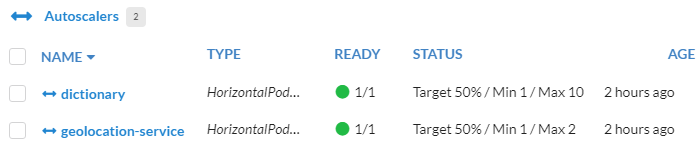
\includegraphics[width=0.9\textwidth]{img/autoscaling/hpa-autoscalers-normal}
	\end{center}
    \caption{Spoczynkowy stan Autoscaler'ów}
\end{figure}

\begin{figure}[!ht]
	\begin{center}
		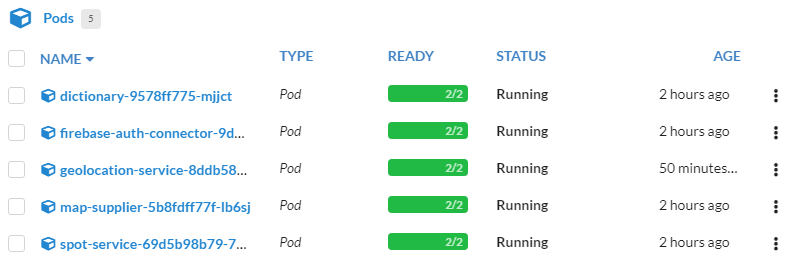
\includegraphics[width=0.9\textwidth]{img/autoscaling/hpa-pods-normal}
	\end{center}
    \caption{Spoczynkowy stan Pod'ów}
\end{figure}

W ramach testu obciążeniowego wysyłany jest za pomocą programu \emph{Postman} nieprzerwany szturm 10 tysięcy zapytań GET o treść jakiegoś słownika:

\begin{figure}[!ht]
	\begin{center}
		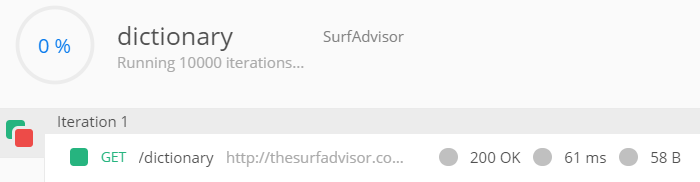
\includegraphics[width=0.8\textwidth]{img/autoscaling/hpa-dictionary-test-postman}
	\end{center}
    \caption{Test obciążeniowy \emph{dictionary-service} z Postmana}
\end{figure}

\cw{Autoscaler}'y reagują po około 10 sekundach zwiększając liczbę \cw{Pod}'ów \emph{dictionary-service}:

\begin{figure}[!ht]
	\begin{center}
		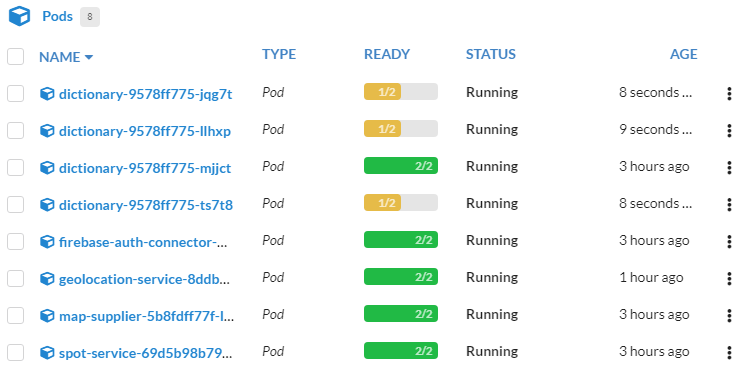
\includegraphics[width=0.9\textwidth]{img/autoscaling/hpa-pods-scale-up}
	\end{center}
    \caption{Stan Pod'ów przy skalowaniu w górę}
\end{figure}

\begin{figure}[!ht]
	\begin{center}
		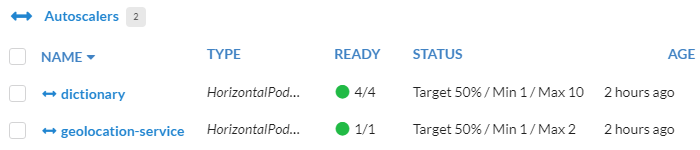
\includegraphics[width=0.9\textwidth]{img/autoscaling/hpa-autoscalers-scale-up}
	\end{center}
    \caption{Stan Autoscaler'ów przy skalowaniu w górę}
\end{figure}

Diagram poniżej pochodzi z konsoli webowej \emph{Grafana} - narzędzia, które wspólnie z \emph{Prometheus} umożliwiają śledzienie metryk technicznych \cw{Cluster}'a.
Przedstawione zostało zużycie CPU poszczególnych \cw{Pod}'ów podczas testu obciążeniowego:

\begin{figure}[!ht]
	\begin{center}
		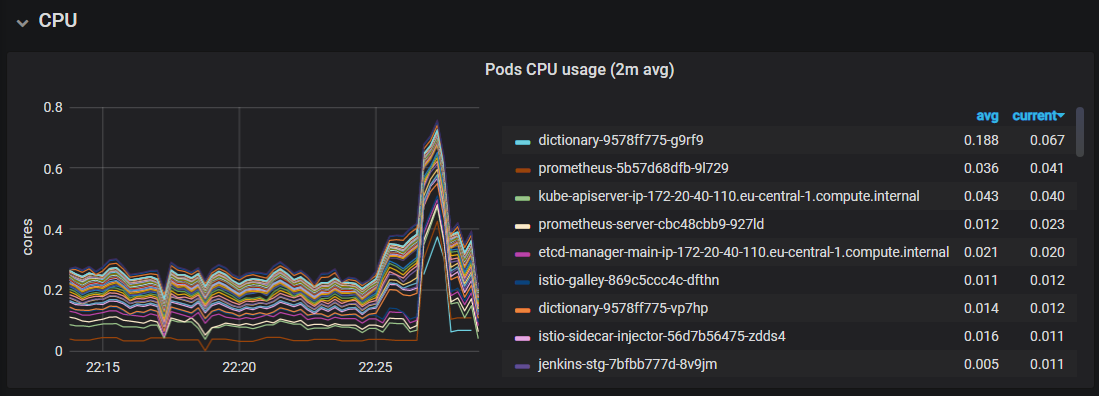
\includegraphics[width=1\textwidth]{img/autoscaling/hpa-grafana-scale-up}
	\end{center}
    \caption{Zużycie CPU podczas testu obciążeniowego \emph{dictionary-service}}
\end{figure}

\section{Horizontal Node Autoscaling}

Z kolei włączenie autoskalowania \cw{Node}'ów jest jeszcze prostsze. 
Ogranicza się do wdrożenia jednej z dostępnych online rekomendowanych definicji \cw{Service}'u \emph{cluster-autoscaler}.
Skalowanie pobudzane jest ilością \cw{Pod}'ów jakie Kubernetes próbuje wdrożyć.
Jeżeli istniejące \cw{Node}'y nie pomieszczą już więcej \cw{Pod}'ów, tworzone są kolejne.


Ilość instancji EC2 w stanie początkowym:

\begin{figure}[H]
	\begin{center}
		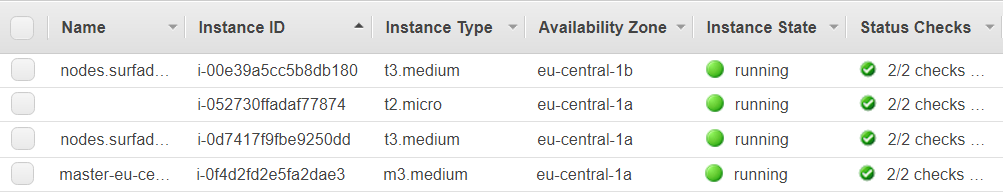
\includegraphics[width=1\textwidth]{img/autoscaling/ca-normal}
	\end{center}
    \caption{Spoczynkowy stan Node'ów}
\end{figure}

Poprzez manualne rozkazy zwiększania ilości \cw{Pod}'ów doprowadzono do przepełnienia \cw{Cluster}'a.
W logach \cw{Service}'u \emph{cluster-autoscaler} zarejestrowana jest reakcja na zastałą sytuację:

\begin{figure}[H]
	\begin{center}
		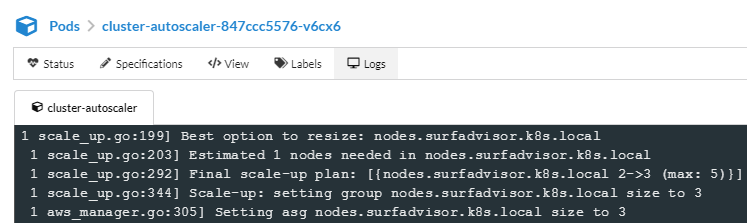
\includegraphics[width=0.9\textwidth]{img/autoscaling/ca-scale-up-logs}
	\end{center}
    \caption{Logi serwisu odpowiedzialnego za skalowanie horyzontalne Node'ów}
\end{figure}

Wynikiem tego działania jest uruchomienie dodatkowej instancji EC2, która rozszerzy pojemność \cw{Cluster}'a i umożliwi wdrożenie wszystkich \cw{Pod}'ów:

\begin{figure}[H]
	\begin{center}
		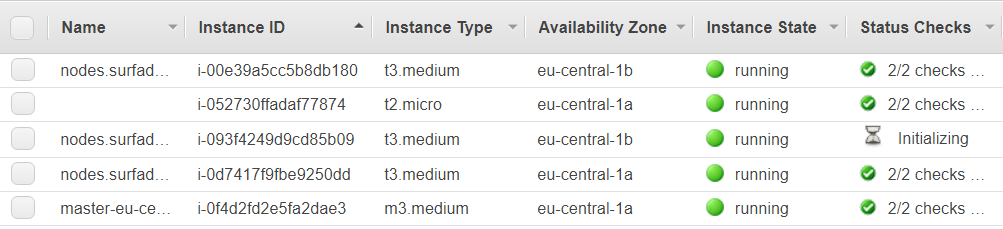
\includegraphics[width=1\textwidth]{img/autoscaling/ca-scale-up}
	\end{center}
    \caption{Stan Node'ów przy skalowaniu w górę}
\end{figure}
